
%!TEX root = ../thesis.tex
%*******************************************************************************
%****************************** Third Chapter **********************************
%*******************************************************************************
\chapter{Reconstructing SBND}
\label{ChapterReco}

% **************************** Define Graphics Path **************************
\ifpdf
    \graphicspath{{Chapter7/Figs/Raster/}{Chapter7/Figs/PDF/}{Chapter7/Figs/}}
\else
    \graphicspath{{Chapter7/Figs/Vector/}{Chapter7/Figs/}}
\fi

%********************************** %Opening  **************************************

Reconstruction is the process of extracting physics quantities from the raw detector data.
For SBND, the goal of reconstruction is to reconstruct particles that deposit energy within the detection subsystems.
A contained particle inside the TPC might deposit energy resulting in only waveforms recorded by the TPC wire planes and the PDS, meanwhile, an exiting particle might deposit addition energy in the CRT walls surrounding the TPC.
For a given particle, the TPC reconstruction is able to extract various quantities describing its topology and charge calorimetry and kinematics.
The PDS reconstruction can provide additional high resolution timing information of the particle on top of its light calorimetry.
The CRT reconstruction can indicate if the particle is fully contained inside the detector.
As a result, the reconstruction variables from all three detection subsystems are complementary to each other can be exploited for different analysis purposes such as cosmic rejection or particle identification. 

This chapter provides a summary of the reconstruction framework at SBND.
The first Sec. \ref{sec:reco_overview} gives an overview of the reconstruction workflow for each detection subsystem. 
The following Sec. \ref{sec:reco_tpc} provides the details of the TPC reconstruction workflow from start to end.
Meanwhile, the reconstruction of the PDS and CRT subsystem will be summarised in Sec. \ref{sec:reco_others}.
Furthermore, descriptions of some high-level analysis tools using the reconstruction variables collectively from each detection subsystems are included in Sec. \ref{sec:reco_ana_tools}.
Finally, the chapter is concluded in Sec. \ref{sec:reco_concluding_remarks} with some remarks.

\newpage

%********************************** %First Section  **************************************

\section{Overview of Reconstructing SBND}
\label{sec:reco_overview}

%Describe the overall workflow
Each detection subsystem in SBND requires a dedicated reconstruction workflow.
An overview of each workflow is illustrated in Fig. \ref{fig:Reco_Workflow}.
The TPC reconstruction workflow is shown by the red boxes.
This process begins with the raw wire waveforms going through the signal processing performed by the Wirecell tool kit \cite{wirecell}.
This is followed by a hit finding algorithm to identify hits on the waveform.
The output hits are then used by the Pandora package \cite{pandora} to output a 3D-reconstructed interaction, denoted as a \textit{slice}.
The PDS reconstruction workflow also follows a similar process to the TPC, shown by the blue boxes.
A waveform deconvolution is first performed on the raw PDS waveforms to filter noise.
Then, a hit finding algorithm identifies optical hits on the waveform and a reconstruction is performed on the hits.
The equivalent output to a TPC-reconstructed interaction from the PDS reconstruction is referred to as a \textit{flash}.
Finally, the reconstruction for the CRTs is much simpler compared to other two subsystems, consisting of only a hit finding and a reconstruction step, as shown in the orange boxes.
The reconstruction variables from each detection subsystem are produced independently and can be matched together if they originate from the same interaction. 
The variables can also be combined and input into different high-level analysis tools to extract more complex properties of the underlying interaction. 

\begin{figure}[htbp!] 
\centering    
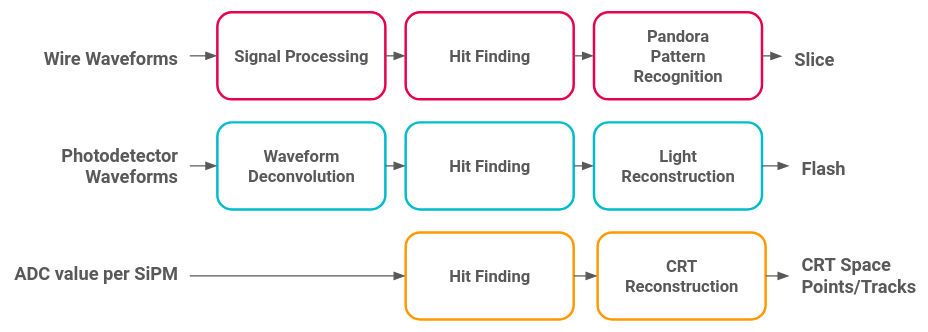
\includegraphics[width=1.0\textwidth]{Reco_Workflow}
\caption[Reco_Workflow]{
Overview of the reconstruction workflow for each detection subsystem of SBND.
}
\label{fig:Reco_Workflow}
\end{figure}

\section{TPC Reconstruction}
\label{sec:reco_tpc}

\subsection{TPC Signal Processing}
%Signal Processing
Signal processing is the first crucial step of TPC reconstruction, which is to deconvolve digitised raw waveforms and remove detector effects such as noise, electronics response and field response. 
At SBND, signal processing is implemented using the WireCell tool kit \cite{wirecell}.
The tool has been used by other various LArTPC experiments such as MicroBooNE and ProtoDUNE and has demonstrated the excellent performance to acquire deconvolved charge by performing deconvolution in time and wire dimension over the traditional deconvolution in time dimension only. 

Fig. \ref{fig:signal_processing_steps} \cite{} demonstrates the step by step of the signal processing.
In grey is the true charge deposition on a wire, and in red is the corresponding raw waveform containing signal convolved with noise, electronics response, field response and noise.
The first step in the chain is noise filtering to remove the excess and correlated noise from raw waveforms.
Then, the measured charge is deconvolved from the electronics and field response to recover the original charge deposited on the wire, as shown in orange.
The deconvolution is 2D, where response functions consider the time response of a single wire as well as responses of neighbouring wires.
This step is particularly important for the induction planes to convert bipolar into unipolar signals, such that the integral of the waveform can be used for charge estimation.
\begin{figure}[tbp!] 
\centering    
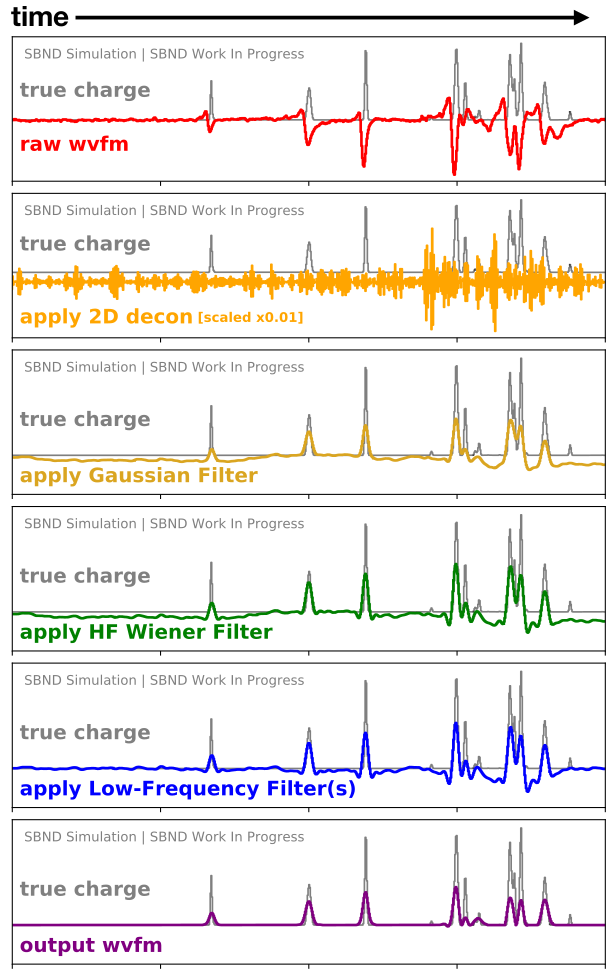
\includegraphics[width=0.45\textwidth]{signal_processing_steps}
\caption[signal_processing_steps]{
Example demonstrating the steps of signal processing applied to a bipolar raw waveform to acquire the final deconvolved waveform.
Fig. from Ref. \cite{}.
}
\label{fig:signal_processing_steps}
%\end{figure}
%\begin{figure}[htbp!] 
\centering    
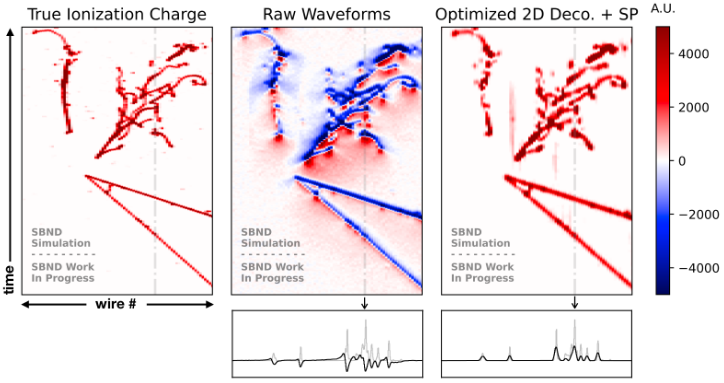
\includegraphics[width=0.75\textwidth]{signal_processing_waveform}
\caption[signal_processing_waveform]{
Event display of a simulated neutrino event using the true ionisation charge (left), raw waveforms (middle) and deconvolved waveforms (right).
Fig. from Ref. \cite{}.
}
\label{fig:signal_processing_waveform}
\end{figure}
Filter functions are applied subsequently to attenuate noise that are artificially amplified.
This includes high frequency filters to remove high frequency noise, where a Gaussian or Weiner filters can be used depending on if the signal is unipolar or bipolar.
Example shown here is a bipolar signal waveform, and therefore has both Gaussian and Weiner filters applied.
Then, low frequency filters are utilised for region-of-interest finding and local baseline removal, shown in blue.
Finally, the deconvolved waveform per wire after baseline removal is shown in purple.

Fig. \ref{fig:signal_processing_waveform} depicts event displays of a simulated neutrino event as recorded by wires on the u plane.
The left event display are made using the true charges on wire, the middle event display is made using raw waveforms and the right event display is made using deconvolved waveforms.
Recently, the deconvolution and filters have been optimised particularly for the SBND detector conditions.
The resulting event display shows clean signals, where two tracks and two showers can be observed, closely resemblance the true charges. 

\subsection{TPC Hit Finding}
After signal processing, hit finding is performed on deconvolved waveforms to search for Gaussian-shaped pulses above a threshold.
This is done by the \texttt{GausHitFinder} module \cite{gaushitfinder} by fitting a series of Gaussians to the waveform.
The number of pulses is determined by the number of maximas found when differentiating the waveform, where each pulse represents a hit.
Fig. \ref{fig:gaushit} \cite{EdPhD} demonstrates the hit finding process for a deconvolved waveform, showing four hits have been identified and fitted with a Gaussian.
Once the hits are fitted, information describing the hit are extracted and used by downstream pattern recognition and reconstruction.
The peak time represents the time at which the charge arrives at the wire, used for determining the drift position and matching hit coincidence across wire planes.
The height and the width of the Gaussian are used to calculate the integral of the pulse, representing thee deposited charge on the wire, subsequently used in downstream analysis for calorimetry computation.

\begin{figure}[htbp!] 
\centering    
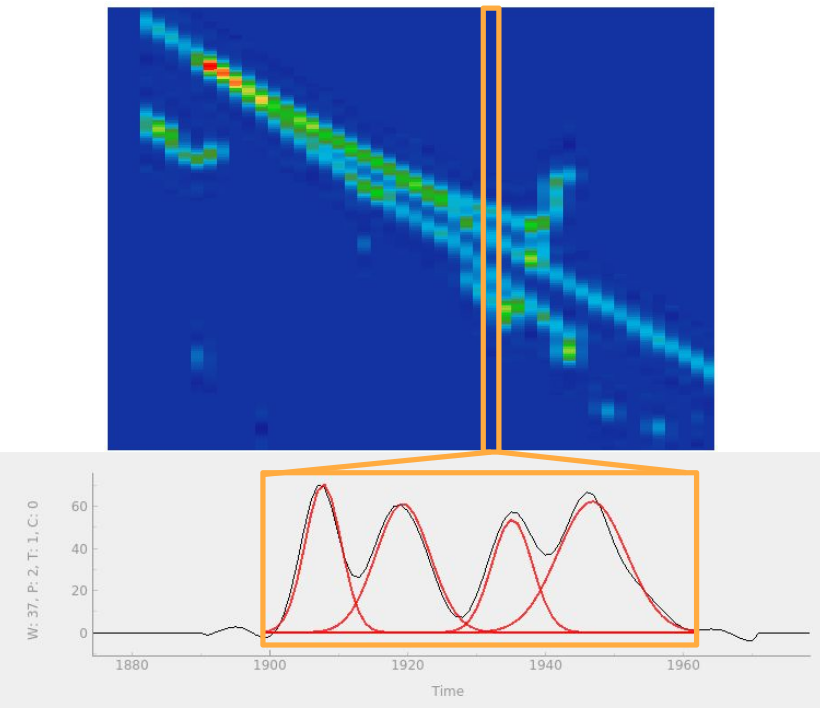
\includegraphics[width=0.55\textwidth]{gaushit}
\caption[gaushit]{
Event display of a simulated neutrino event, and a using the true ionisation charge (left), raw waveforms (middle) and deconvolved waveforms (right).
Fig. from Ref. \cite{EdPhD}.
}
\label{fig:gaushit}
\end{figure}

\subsection{Pandora Pattern Recognition}

%Pattern Recognition: Pandora
The output hits from the hit finding process are then used to perform 3D reconstruction, which is performed with the Pandora pattern recognition package\cite{pandora}. 
The package was first developed for the International Linear Collider, and later extended to other LArTPC experiments.
It is made up of over 100 individual algorithms, performing a specific task along the reconstruction chain.
The output from Pandora represents an interaction, containing a hierarchy of particles starting with a neutrino parent at the interaction vertex.
This reconstructed object is referred to as a \textit{slice}.  

The reconstruction begins with a workflow to reconstruct cosmic-like objects that leave long tracks inside the detector.
This workflow performs a 2D clustering on each wire plane independently, followed by 3D reconstruction under the assumption that all clusters are track-like.
Then, a cosmic rejection is performed to to identify if a cluster is cosmic-like or neutrino-like.
The cosmic removal at this stage is deliberately cautious such that only very unambiguous cosmic muons in nature are removed.

The remaining clusters are then input into a second workflow dedicated towards neutrino reconstruction.
This workflow begins with a slicing algorithm that divides the clusters into \textit{slices}, where each slice encapsulates hits coming from a single origin, representing an interaction.
Then, 2D clustering is re-performed on each wire plan independently, however, with a new assumption that clusters can be both track-like and shower-like.
A vertexing algorithm then identifies the interaction vertex of the slice and its associated clusters.
A series of pattern matching algorithms grows the interaction out of a neutrino vertex, and performs 3D reconstruction by matching 2D clusters across different planes.
The output 3D reconstructed object associated with a vertex ideally represent a \textit{particle} produced from an interaction.

At this stage, a track score is assigned to a particle if it has a track-like or a shower-like topology, which is determined by a dedicated Boosted Decision Tree (BDT).
The development work on the track and shower separation BDT and its importance not only in the reconstruction workflow but also in the analysis workflow will be covered in the next Sec. \ref{sec:trkshwbdt}.
Both track and shower reconstruction tools are then performed on the particle under the assumption if it is track-like or shower-like respectively. 
Finally, a hierarchy algorithm is performed to classify the hierarchy of particles in a slice, starting with a neutrino parent vertex, and other particles are children, grandchildren, etc. of the parent.

%Calorimetry reconstruction
The last stage of reconstruction is calorimetry computation for the output slices, and its associated particles.
Both track and shower calorimetry computations first convert ADC units to charge, or number of electrons, via multiplying a charge calibration constant.
The track calorimetry then computes the energy from charge using the Argoneut-parametrised ModBox recombination formalism, factoring in the electric distortion due the space charge effect.
Meanwhile, the shower calorimetry reconstruction converts the measured charge to energy by multiplying a shower calibration constant.
Once the SBND detector is operational, the calibration constants will be measured via dedicated calibration physics runs.
The charge calibration constant is expected to be computed from using a sample of anode to cathode crossing muon tracks while the shower calibration constant can be acquired from using standard candle of the neutral pion invariant mass \cite{}.

\subsection{Track-Shower Separation Boosted Decision Tree}
\label{sec:trkshwbdt}
As previously discussed, reconstructed particles from Pandora are assigned with a track score determined by Boosted Decision Tree (BDT), which is a binary classification machine learning tools.
The track score spans between 0 and 1 such that if a particle has a very high track score close to 1, then the particle is track-like.
Otherwise, if the track score is very close to 0, then the particle is shower-like.

The track-shower BDT has become more important in the reconstruction as well as the analysis workflow due to a new reconstruction paradigm introduced by Pandora.
The traditional reconstruction approach was to perform only either track or shower reconstruction on a particle based on its track score.
Meanwhile, the new paradigm performs both track and shower reconstruction on a particle regardless of the track score.
All reconstructed particles now have two sets of reconstruction variables for track-like and shower-like.
The analyzers have the freedom to decide which variables to use depending on their signal topology, and thus not pre-determined by Pandora.
The track score provides the necessary information if the signal topology is more track-like or shower-like and therefore, which appropriate reconstruction variables should be used for the analysis. 

The track-shower BDT was trained trained on series of reconstruction variables, has been recently updated to include new variables for the training.
The original BDT includes variables describing the geometrical topology of the particle such as its length, distance and direction with respect to the parent vertex, as well as calorimetry variables describing the charge distribution of the particle.
More details of the input variables and the training of the BDT can be found in Ref. \cite{EdPhD}.
The update extended beyond the original work to include a brand new set of variables describing how cone-like the charge distribution of a particle as well as a new set of variables describing the particle hierarchy.

The cone variables were first developed by the Pandora Warwick team \cite{}, which consist of three variables: (1) Halo total ratio, (2) concentration and (3) conicalness as depicted in Fig. \ref{fig:cone_variables}.
The diagrams depict hit distribution of a hypothetical particle, where each circle represents a hit associated with a charge value and the star represents the neutrino vertex.
The illustration is in 2D however the variables are computed in 3D.
The first variable is the halo-total ratio, illustrated in Fig. \ref{fig:halototalratio}.
The region outside of the Moliere radius, defined such that 90\% of the cluster energy is contained within this radius, is considered the halo region.
The halo hits are shown as green circles whereas hits inside the Moliere radius are shown as grey circles.
The halo-total ratio is then defined as 
\begin{equation}
	Halo\ Total\ Ratio = \frac{Charges\ in\ The\ Halo}{Total\ Charges}
\end{equation}
The second variable is called concentration, accounting for how concentrated the charge distribution to the centre of the cluster.
This is depicted in Fig. \ref{fig:concentration}, where each hit is assigned with a colour showing how weighted it is with respect to its orthogonal distance to the cluster direction.
The closer the hit to the centre, the more weighted it is.
The concentration variable is defined the total weighted charges divided by the total charge as following
\begin{equation}
	Concentration = \frac{\sum Charge \times Weight}{Total\ Charges}
\end{equation}
Finally, the conicalness variable examines the hit distribution at the end and the start of the cluster as depicted in Fig. \ref{fig:conicalness}. 
It is defined the ratio between the concentration at the end of the cluster compared to at the start of the cluster
\begin{equation}
	Conincalness = \frac{Concentration\ at\ The\ End}{Concentration\ at\ The\ Start}
\end{equation}
\begin{figure}[htbp!]
        \centering
        \begin{subfigure}[b]{0.495\textwidth}
            \centering
            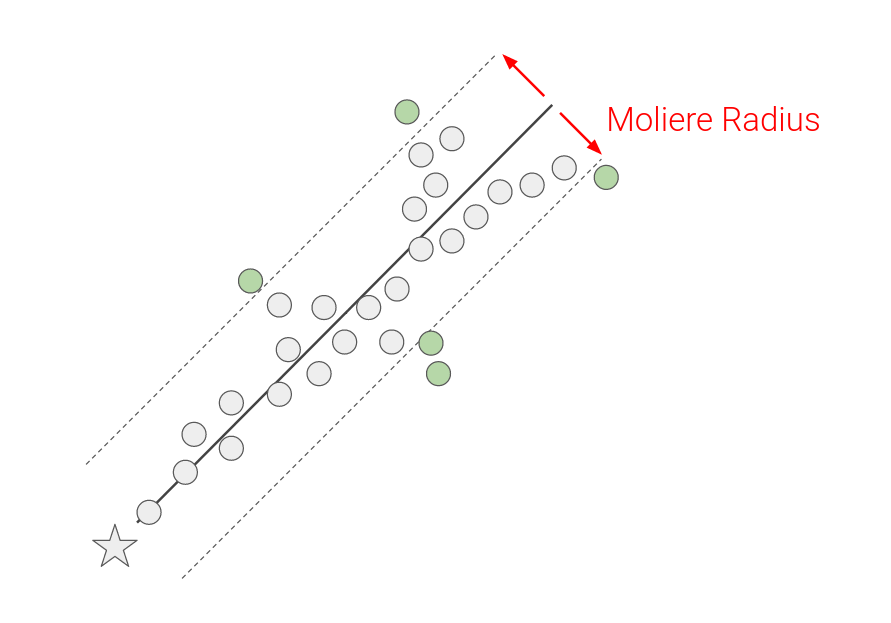
\includegraphics[width=\textwidth]{HaloTotalRatio}
            \caption{Halo Total Ratio}%
            \label{fig:halototalratio}
        \end{subfigure}
        \hfill
        \begin{subfigure}[b]{0.495\textwidth}  
            \centering 
            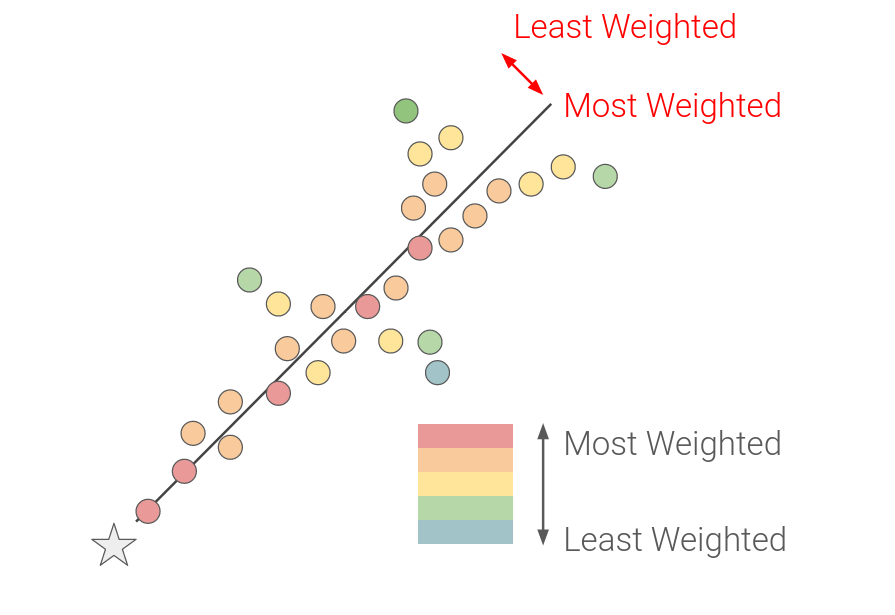
\includegraphics[width=\textwidth]{Concentration}
            \caption{Concentration}%
            \label{fig:concentration}
        \end{subfigure}
        \hfill
        \begin{subfigure}[b]{0.495\textwidth}  
            \centering 
            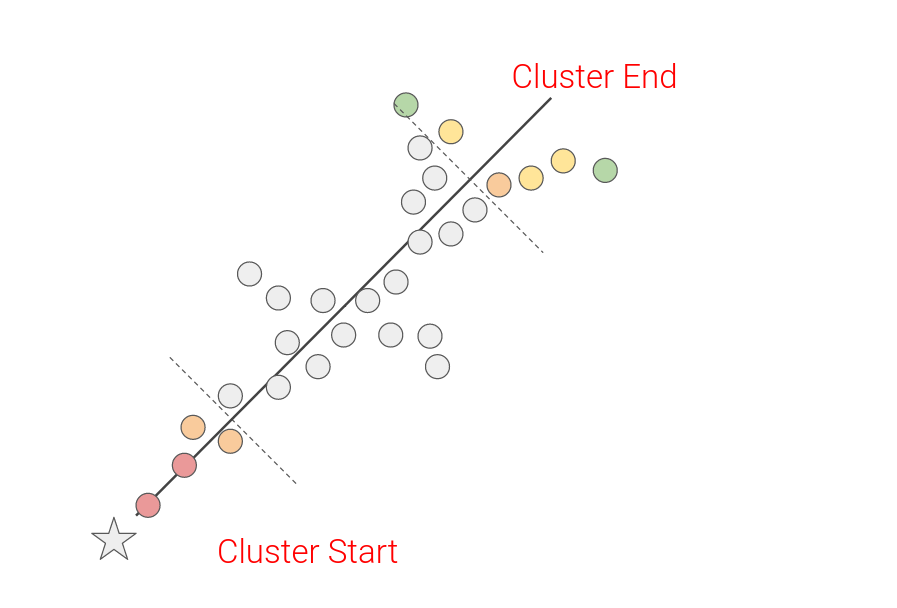
\includegraphics[width=\textwidth]{Conicalness}
            \caption{Conicalness}%
            \label{fig:conicalness}
        \end{subfigure}
        \caption[cone_variables]{
	Diagrams illustrating the variables describing how cone-like the charge distribution of a particle .
	}
        \label{fig:cone_variables}
\end{figure}

One new variable introduced to the track-shower separation BDT that describes the hierarchy of the particle within the reconstructed interaction or slice.
For a given particle, the daughters originating from that particle are identified and their number of hits are counted.
The distributions of the four new variables for a track-like and shower-like particle are shown in Fig. \ref{fig:bdt_features}.
The concentration and conicalness variables display the strongest separation power between tracks and showers compared to the halo total ratio and the number of daughter hits variables.

\begin{figure}[htbp!]
        \centering
        \begin{subfigure}[b]{0.45\textwidth}
            \centering
            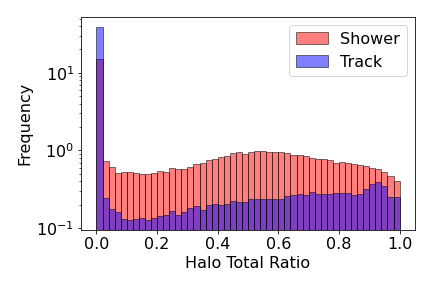
\includegraphics[width=\textwidth]{Feature_Halo_Total_Ratio}
            \caption{Halo Total Ratio}%
            \label{fig:feature_halototalratio}
        \end{subfigure}
        \hfill
        \begin{subfigure}[b]{0.45\textwidth}  
            \centering 
            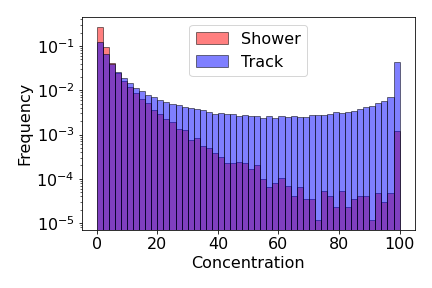
\includegraphics[width=\textwidth]{Feature_Concentration}
            \caption{Concentration}%
            \label{fig:feature_concentration}
        \end{subfigure}
        \hfill
        \begin{subfigure}[b]{0.45\textwidth}  
            \centering 
            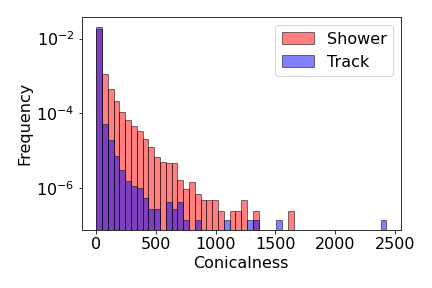
\includegraphics[width=\textwidth]{Feature_Conicalness}
            \caption{Conicalness}%
            \label{fig:feature_conicalness}
        \end{subfigure}
        \hfill
        \begin{subfigure}[b]{0.45\textwidth}  
            \centering 
            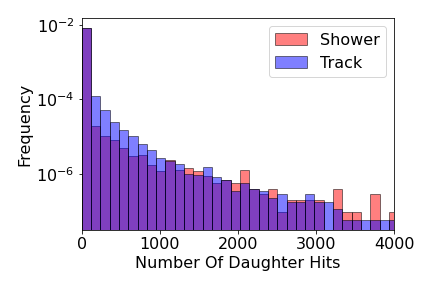
\includegraphics[width=\textwidth]{Feature_Number_Of_Daughter_Hits}
            \caption{Number of Daughter Hits}%
            \label{fig:feature_nDaughterHits}
        \end{subfigure}
        \caption[bdt_features]{
	Distributions of the new variables input into the track-shower separation BDT, plotted for track-like and shower-like particles.
	}
        \label{fig:bdt_features}
\end{figure}

Fig. \ref{fig:bdt_score} shows the score distribution of the BDT retrained with the four new variables.
The left figure shows two distinct distributions in red and blue for showers and tracks respectively.
This demonstrates a good separation power of the BDT, where particles with score less than 0.5 closely resemblance showers whilst particles with score more than 0.5 are more track-like.
The score distribution is broken down into different particle type as shown in the right figure.
The distribution is expected given that electrons and photons leave electromagnetic shower activities inside the detector whilst charged particles like muons, pions and protons leave track-like signatures. 
The updated BDT resulted in $0.1\sim2.0\%$ improvement in correctly classifies particle type as shower-like or track-like.
The track-shower separation score distribution will be used in downstream high level analysis tools, to be detailed in Sec. \ref{sec:subsystem_match}, as well as will be employed as a cut variable in the HNL selection, to be detailed in Sec. \ref{}.

\begin{figure}[htbp!]
        \centering
        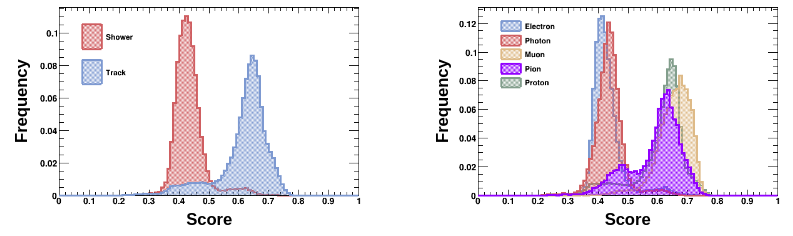
\includegraphics[width=\textwidth]{bdt_score}
        \caption[bdt_score]{
	Score distribution of the updated track-shower separation BDT, plotted for track-like and shower-like particles (left) and plotted for individual particle type (right).
	}
        \label{fig:bdt_score}
\end{figure}

\section{Other Subsystems Reconstruction}
\label{sec:reco_others}

\subsection{PDS Reconstruction}

The reconstructions for the photodetectors, PMTs and X-ARAPUCAs, share the same steps of waveform deconvolution, hit finding and light reconstruction.
However, different algorithms and parameters settings are required for each photodetector type due to their difference in response.
More details on the PDS reconstruction at the SBND detector can be found in Ref. \cite{}.
The following focuses more on the reconstruction of PMTs which has an averaged Single Electron Response (SER) pulse peaking at $\sim 25$ ADC and a full width at half maximum of $\sim$ 10 ns.
The fast response of PMT plays the key role in the nanosecond timing resolution requirement for the HNL search.

Similarly to the signal processing in TPC reconstruction, the PMT waveform deconvolution also aims to remove noise and determine the waveform baseline.
Fig. \ref{fig:pds_reco_deconvolution} \cite{} depicts an example PMT waveform before and after the deconvolution.
The top figures shows the MC photons arrived at a given PMT in green.
The middle figure shows the simulated raw PMT waveform in blue, convolved with PMT response and noise.
The AC circuits of the PMTs lead to over/undershoots features across the waveform with respect to the baseline shown in red.
The waveform deconvolution step consists of a 1D deconvolution and an application of Gaussian filter to remove high frequency noise.
The resulting waveform is shown in orange in the bottom figure.
The bipolarity of the signals are fully removed while the integral and temporal position of the peaks are well-maintained.

\begin{figure}[tbp!]
        \centering
        \begin{subfigure}[b]{0.59\textwidth}
            \centering
            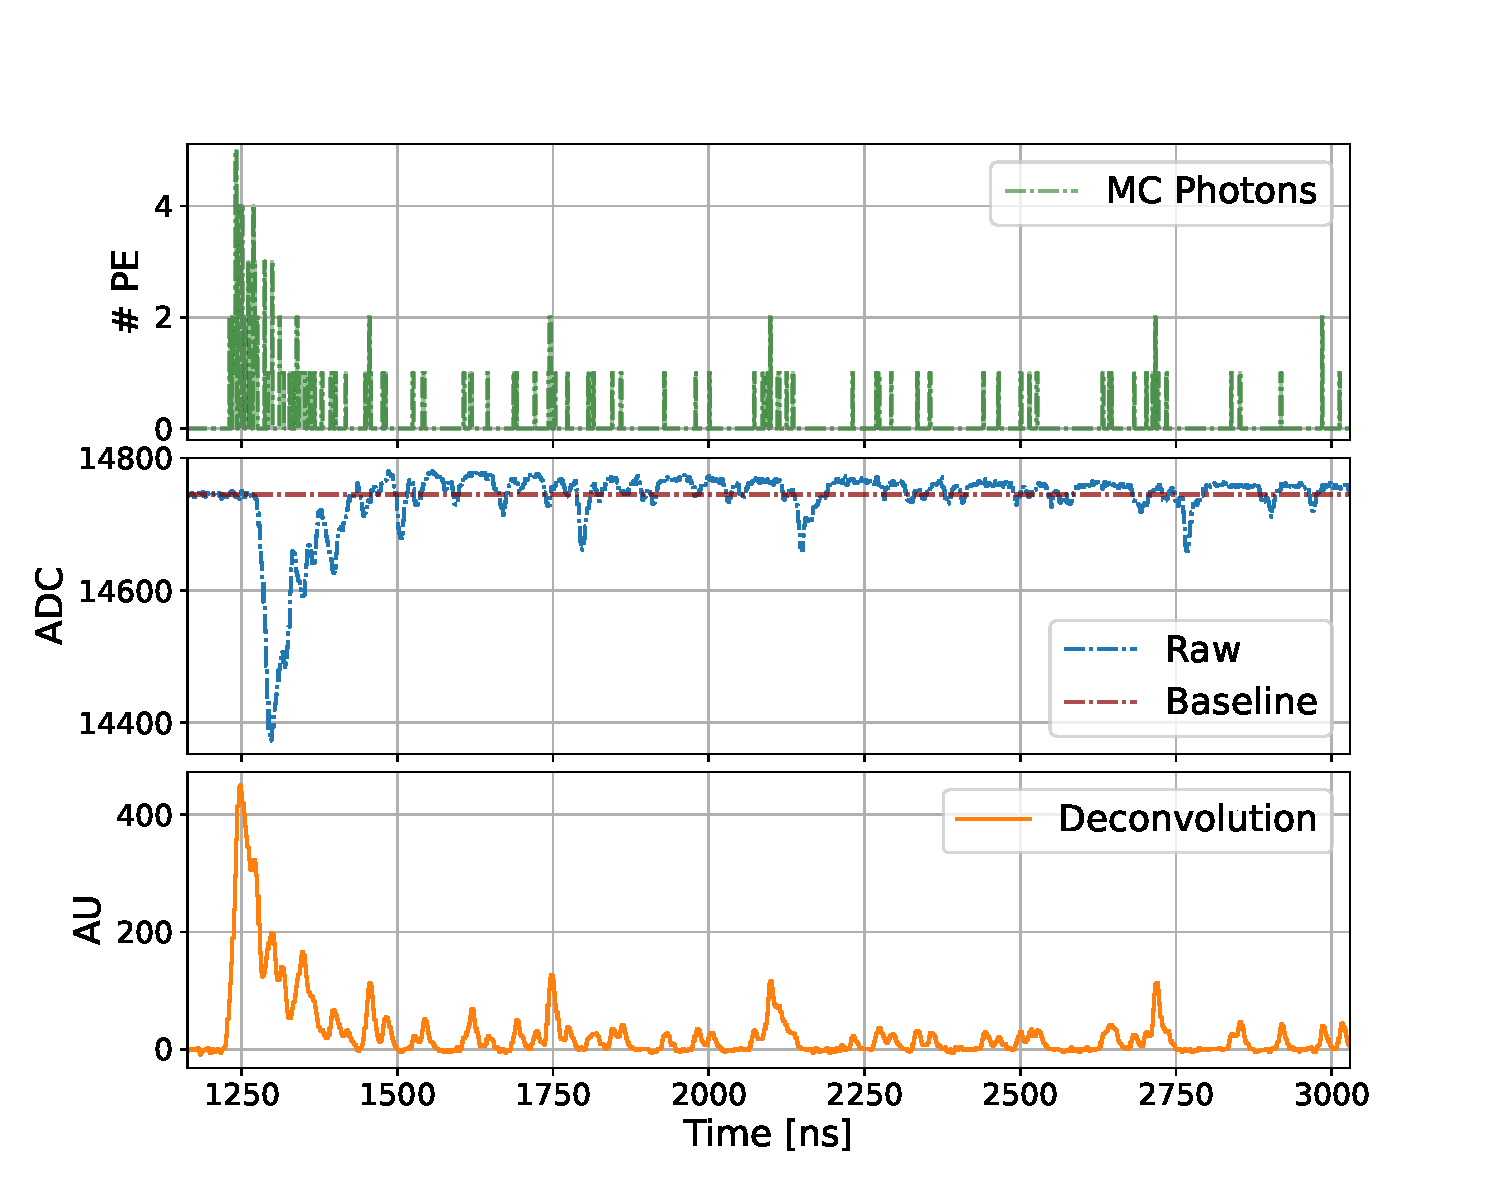
\includegraphics[width=\textwidth]{pds_reco_deconvolution}
            \caption{Waveform Deconvolution}
            \label{fig:pds_reco_deconvolution}
        \end{subfigure}
        \hfill
        \begin{subfigure}[b]{0.4\textwidth}  
            \centering 
            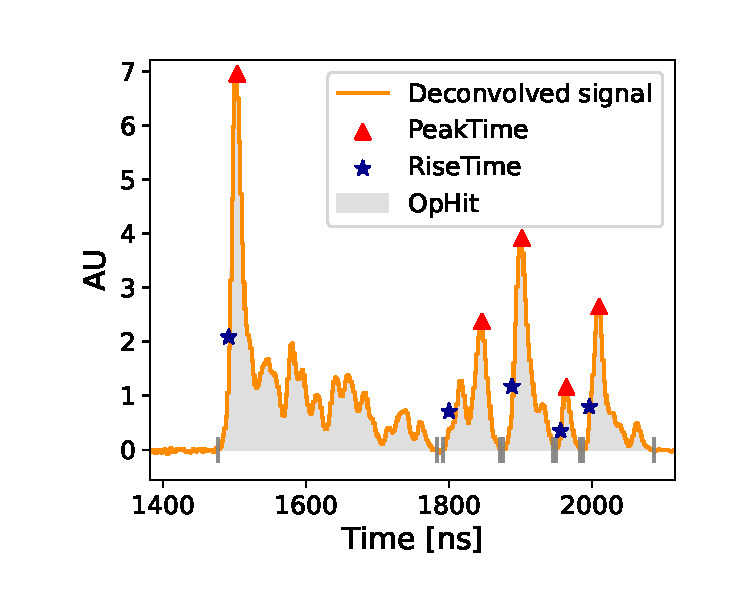
\includegraphics[width=\textwidth]{pds_reco_hit_finding}
            \caption{Hit Finding}
            \label{fig:pds_reco_hit_finding}
        \end{subfigure}
        \caption[pds_reco]{
	Examples 
	Both figures from Ref. \cite{}.
	}
        \label{fig:pds_reco}
\end{figure}

Then, the next step is to perform hit finding on the deconvolved PMT waveform as demonstrated in Fig. \ref{fig:pds_reco_hit_finding}.
The hit finding begins with a baseline subtraction, which is calculated using a 400 ns portion at the start and end of the deconvolved waveform, resulting in the waveform shown in orange.
Optical hits are identified by finding pulse goes above a threshold of $1/4$ the amplitude of the deconvolved SER and 3 standard deviations away from the baseline RMS.
The example shows 4 identified optical hits, with peak times denoted with red triangles.
The first optical hit contains multiple peaks merged into a single optical hit due to multiple photons arrive very closely to the PMT.
The rise time of an optical hit is then estimated as the time at which the pulse goes above 15\% of the peak  amplitude, denoted with blue stars, results in a resolution of 1.6 ns  in estimating the arrival time of the first photon contributing to the optical hit.
The integral of the optical hit are then computed to estimate the number of photoelectrons (PEs) of the hit.

After the hit finding, the light reconstruction algorithm then clusters optical hits into an \textit{optical flash}.
The length of an optical flash is set as 8 $\mu$s to account for the total light produced in an interaction, from both prompt and slow components of scintillation photons.
The clustering algorithm is based on several conditions on the calorimetry of the hits, timing distribution between hits and geometrical location of the PMTs.
The number of PEs in an optical flash is the sum of PEs of optical hits clustered in that flash, ideally represent the total light generated by an interaction. 

The start time of the optical flash represents the start time of an interaction, $t_0$, which is the key variable of the HNL search, and therefore requires great care in reconstruction.
The flash start time is the average of the rise time of optical hits in a flash for the PMTs that contribute 50\% of the prompt light in the 30 ns window of the largest PE pulse. 
Then, a correction is applied for the propagation of the photons from the scintillation position in the TPC to the PMTs, i.e. in the drift or $x$-direction.
This can done by exploiting the high density of PMTs as well as having PMTs sensitive to either or both direct and reflected light component.
As previously shown in Fig. \ref{fig:light_yield_Diego} with some discussions in Sec. \ref{sec:wls}, the arrival time distribution for the direct VUV and reflected visible photons varies with the drift distance.
For a given scintillation position, and therefore a drift position, the resulting amount of direct and visible photons can lead to a specific ratio of the two components seen by the PMTs.
And therefore, the ratio of the number of photons seen by TPB-coated PMTs to those seen by the uncoated PMTs can be used to compute the correction for the propagation effect.
The timing resolution of the flash time after propagation correction varies $\sim 2$ ns across the entire drfit distance, demonstrating the excellent capability of the PDS at SBND.

\subsection{CRT Reconstruction}

The reconstruction workflow for the CRT subsystem is the simplest compared to the TPC and the PDS procedure.
As previously detailed, the output data of the CRT readouts are in group of 32 ADC values, for a single ADC per SiPM.
The reconstruction begins with a hit finding algorithm to identify which pair of SiPM in the group of 32 goes above a threshold.
The SiPM pair determines the lateral position of a cosmic muon hit within a CRT strip.
Then, a clustering algorithm groups hits from orthogonal CRT strips of the same wall within a 50 ns window to yield 3D space points.
For each CRT space point, the timing and calorimetry information is calculated and corrected for the propagation effect due to the longitudinal distance from the hit position to to the SiPM.
The final step of the reconstruction is to match space points from multiple CRT walls to form a CRT track.
Candidate tracks are evaluated from any combinations of space points from different taggers within a 100 ns coincidence window.
The best track candidate is selected by the goodness of timing agreement and prioritising three-point tracks over two-point tracks. 
The outputs of the CRT reconstruction are both CRT space points and CRT tracks. 

%********************************** %First Section  **************************************
\section{High-Level Analysis Tools}
\label{sec:reco_ana_tools}

The reconstructed variables from each detection subsystems, slices from the TPC, flashes from the PDS, space points and tracks from the CRTs, can then be used collectively by downstream algorithms to compute useful information regarding the interaction.
The following section covers the main high-level analysis tools used in the HNL search, and the details of their usage will be discussed in Sec. \ref{}.
Firstly, Sec. \ref{sec:subsystem_match} provides the details on how variables from different detection subsystems can be matched to the same interaction.
Moreover, Sec. \ref{sec:crumbs} discusses the tools used to perform cosmic rejection, which is an abundant background due to SBND being an overground detector.
Finally, Sec. \ref{sec:razzled} illustrates the tools used for particle identification. 

\subsection{Subsystems Matching Tools}
\label{sec:subsystem_match}

The reconstructed tracks using the TPC can be matched to a space point or tracks from the CRTs to provide additional information for cosmic rejection.
An example is that a through going cosmic ray produces a long track in the TPC as well as deposit energy in the nearest CRT walls where the TPC tracks starts and ends. 
Another example is that tracks produced in the TPC deposits energy in the nearest CRT strips only when enters or exits the detector, enabling the tagging of stopping cosmic muons or exiting neutrinos.

Two types of matching are performed: (1) matching TPC track to CRT space point and (2) matching TPC track to CRT track.
The former method extrapolates the TPC track and matches with the nearest CRT space point by computing a distance of closest approach (DCA), confining the matching to a single CRT wall.
The latter method uses a compound score from the average DCA stepping along the TPC track and the angle between the TPC and CRT tracks, enabling matching a single TPC track to two or more CRT walls.
Both method uses the timing information of the CRT objects for further constraints and no duplications are in matching are allowed.

The second subsystem matching of interest is matching an interaction reconstructed using the TPC wires, a slice, to an interaction reconstructed using the PDS, a flash.
This matching is vitally important given that the flash time is the nanosecond resolution timing variable.
A flash time matched to a slice represents the start time of the interaction reconstructed in that slice, and therefore the key variable separating the showers resulting from HNL decays from other SM observables.

The matching of the TPC to the PDS is done with the module \texttt{Opt0Finder} \cite{}.
The basis of the matching is on the estimation of charge yield in a slice seen by the wires to predict the expected light yield seen by the PMTs.
For a given slice, the module first calculates the charge yield to energy to light yield in a slice based on their topology.
The track score of the particles in the slice, that assigned by the track-shower separation BDT detailed in Sec. \ref{sec:trkshwbdt}, is used here to indicate whether the particle is track-like or shower-like and therefore which appropriate calorimetry computation to use.
If the particle is track-like, the calorimetry computation uses the ModBox recombination formalism with the charge-light anti-correlation. 
Otherwise, the calorimetry computation uses a charge to light conversion by multiplying a constant.
Then, from the estimated light yield, the module constructs a hypothesis to compute the number of PE seen by each PMT by re-running the semi-analytical light library.
Finally, the hypothesis PE is compared to the actual measured PE for any given flashes through a $\chi^2$ minimisation.
The flash that is best matched to a slice is the one with lowest $\chi^2$.
At the moment, the module can only match a single optical flash to a slice.

A useful variable output from this matching process is the comparison between the hypothesis PE to the measured PE in the matched flash.
This variable is defined as Opt0 fraction as follows
\begin{equation}
\label{eq:opt0fraction}
Opt\textit{0}\ fraction = \frac{Hypothesis\ PE - Measured\ PE}{Measured PE}
\end{equation}
This indicates the level of agreement of the number of PE hypothesised from deposited charge in a slice relative to the number of PE measured in the matched flash.
If the fraction is positive, the hypothesis is overestimated, otherwise, the hypothesis is underestimated.
This variable is particularly useful in the selection of HNLs to be detailed in Sec. \ref{}, where it does not only provide calorimetry information from both the TPC and PDS but also their level of agreement.

\subsection{Cosmic Rejection Tools}
\label{sec:crumbs}

The Cosmic Rejection Using a Multi-system Boosted decision tree Score (CRUMBS) aims to exploit all three detection subsystems of SBND to reject cosmic.
This is a binary classification machine learning tools that output score whether a reconstructed slice, or an interaction, is cosmic-like or neutrino-like. 
CRUMBS takes reconstruction inputs from all three detection subsystems, TPC, PDS and CRTs that are complementary to each other, and therefore vastly reduces inefficiencies compared to using a single system.
The TPC information includes reconstructed variables treating a particle as both neutrino-like and cosmic-like, accounting for its topology distribution, geometrical location within the detector and calorimetry.
The PDS information is from the flash best matched to the slice of interest, particularly the number of PEs in the flash and the $\chi^{2}$ discriminant from the matching minimisation.
Finally, the CRT information contains the outputs from both TPC-CRT matching algorithms, accounting for the timing for the CRT space point/track and the matching score.
CRUMBS was trained using the TMVA toolkit \cite{tmva} on MC samples of neutrinos, evenly distributed between $CC\nu_{\mu}$ and $CC\nu_{e}$, and cosmic muons.
The score distribution of CRUMBS shows a significant separating power between neutrino-like signal and cosmic-like background.
Similar to the track-shower separation BDT, a cut can be placed on the score distribution to reject cosmics, with more details provided in Sec. \ref{}.

\subsection{Particle Identification Tools}
\label{sec:razzled}

The main tools for particle identification in the HNL search is called Razzled, which is a multi-classification BDT designed to identify particle type that would deposit energy inside SBND: $e$, $\gamma$, $\mu$, $\pi$ and $p$.
Razzled was also implemented using the TMVA toolkit \cite{tmva}.
The reconstruction variables input into the Razzled are only from using TPC reconstruction variables, particularly from Pandora package where track-like and shower-like reconstruction are both performed on the same particle.
There are three categories of the reconstruction variables input for training Razzled: (1) generic reconstruction variables, (2) track-like variables and (3) shower-like variables.
The generic variables describe the particle multiplicity, topology directionality and charge distribution.
Track reconstruction variables include track length, calorimetry, stopping $\chi^{2}$ ratio to identity Bragg peak, and Multiple Coulomb Scattering (MCS) for muon-pion separation.
Shower reconstruction variables include shower conversion gap, opening angle and calorimetry aiming towards photon-electron separation.
A full description of the input variables can be found in Ref. \cite{EdPhD}.
By combining a collection of variables, Razzled exploits correlation between variables, significantly improving the identification performance over traditional hand cuts.
For each reconstructed particle, Razzled BDT outputs a score for each particle type and assigns the highest particle type score to that particle.

\section{Concluding Remarks}
\label{sec:reco_concluding_remarks}

The overall reconstruction workflow of SBND has been described, outlining the reconstruction process for each detection system, TPC, PDS and CRTs.
The three detection subsystems together provides complementary information regarding the underlying reconstructed interaction, and have been used collectively by different analysis tool for different purposes.
Particularly for the HNL search, the background rejection and signal selection will be based a combination of variables and tools employing all three subsystems in order to achieve a high signal to noise ratio, as will be discussed in the forth coming Chapter \ref{ChapterSelect}.
